%% Charlie Redmon
%% 20171019
%% SEM path diagram

% standalone class for individual image to be included in a document
% border=15pt controls the whitespace padding around the diagram
\documentclass[border=15pt]{standalone}

% additional packages
\usepackage{amsmath}

% load custom style configurations from separate file
%% ------------------------------------------------------------
%% Charlie Redmon
%% 20170923
%% semTikzStyle.tex: style configurations for SEM path diagrams
%% ------------------------------------------------------------

\usepackage{tikz}

% observed variable
\tikzstyle{ov}=[shape=rectangle,
                draw=black!80,
                minimum height=0.6cm,
                minimum width=0.6cm,
                thick]

% response variable
\tikzstyle{av}=[shape=rectangle,
                draw=black!80,
                fill=black!10,
                minimum height=0.6cm,
                minimum width=0.6cm,
                thick]

% latent variable
\tikzstyle{lv}=[shape=circle,
                draw=black!80,
                thick,
                minimum width=1cm]

% correlations
\tikzstyle{lcor}=[bend left=30, dashed]
\tikzstyle{rcor}=[bend right=30, dashed]

% self-loops (for variance)
\tikzstyle{lloop}=[loop left, 
                   out=210, 
                   in=150, 
                   distance=0.3cm,
                   densely dotted]

\tikzstyle{rloop}=[loop right, 
                   out=30, 
                   in=-30, 
                   distance=0.3cm,
                   densely dotted]

\tikzstyle{aloop}=[loop above, 
                   out=60, 
                   in=120, 
                   distance=0.3cm,
                   densely dotted]

\tikzstyle{bloop}=[loop below, 
                   out=-60, 
                   in=-120, 
                   distance=0.3cm,
                   densely dotted]




\usetikzlibrary{positioning, calc, arrows.meta}


\begin{document}

%% ">=Latex" sets the arrow head style
%% "semithick" sets the line width (0.6 pt)
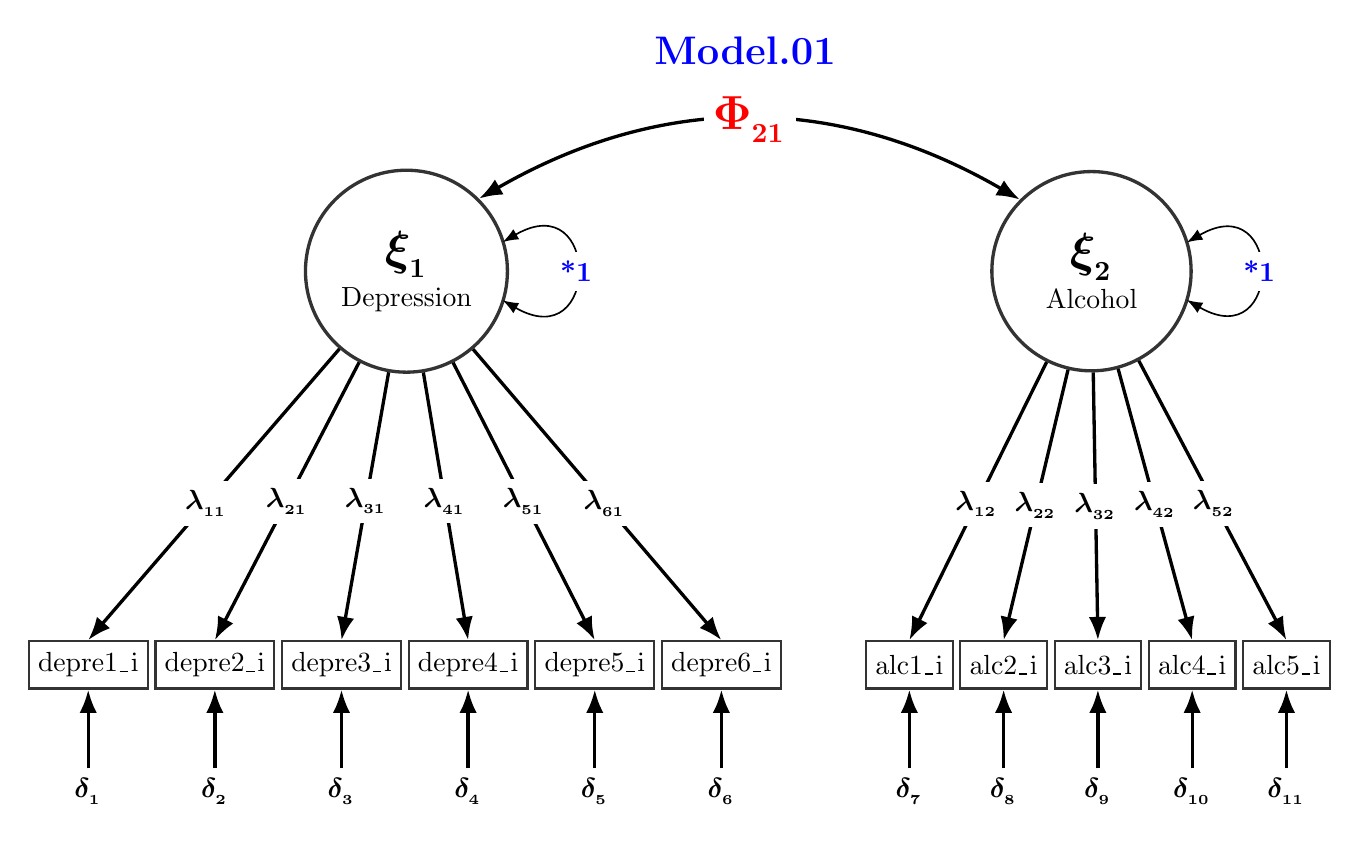
\begin{tikzpicture}[>=Latex, semithick]

% observed variables
\node[ov] (d6) at (0,0)  {depre6\_\hspace{0.1em}i};
\node[ov, left=0.2em of d6] (d5) {depre5\_\hspace{0.1em}i};
\node[ov, left=0.2em of d5] (d4) {depre4\_\hspace{0.1em}i};
\node[ov, left=0.2em of d4] (d3) {depre3\_\hspace{0.1em}i};
\node[ov, left=0.2em of d3] (d2) {depre2\_\hspace{0.1em}i};
\node[ov, left=0.2em of d2] (d1) {depre1\_\hspace{0.1em}i};

\node[below=of d6] (delt6) {$\boldsymbol{\delta_{_6}}$};
\node[below=of d5] (delt5) {$\boldsymbol{\delta_{_5}}$};
\node[below=of d4] (delt4) {$\boldsymbol{\delta_{_4}}$};
\node[below=of d3] (delt3) {$\boldsymbol{\delta_{_3}}$};
\node[below=of d2] (delt2) {$\boldsymbol{\delta_{_2}}$};
\node[below=of d1] (delt1) {$\boldsymbol{\delta_{_1}}$};


\node[ov, right=3em of d6] (a1) {alc1\_\hspace{0.1em}i};
\node[ov, right=0.2em of a1] (a2) {alc2\_\hspace{0.1em}i};
\node[ov, right=0.2em of a2] (a3) {alc3\_\hspace{0.1em}i};
\node[ov, right=0.2em of a3] (a4) {alc4\_\hspace{0.1em}i};
\node[ov, right=0.2em of a4] (a5) {alc5\_\hspace{0.1em}i};

\node[below=of a1] (delt7) {$\boldsymbol{\delta_{_7}}$};
\node[below=of a2] (delt8) {$\boldsymbol{\delta_{_8}}$};
\node[below=of a3] (delt9) {$\boldsymbol{\delta_{_9}}$};
\node[below=of a4] (delt10) {$\boldsymbol{\delta_{_{10}}}$};
\node[below=of a5] (delt11) {$\boldsymbol{\delta_{_{11}}}$};

% latent variables
\node[lv, minimum width=2.5cm, text width=2cm, align=center, very thick] (f1) at (-4, 5) {\LARGE $\boldsymbol{\xi_{_1}}$ \\[0.2em] {\normalsize Depression}};
\node[lv, minimum width=2.5cm, text width=2cm, align=center, very thick] (f2) at (4.7, 5) {\LARGE $\boldsymbol{\xi_{_2}}$ \\[0.2em] {\normalsize Alcohol}};


% paths
\path[->, very thick] (f1) edge node[fill=white, pos=0.53] {$\boldsymbol{\lambda_{_{61}}}$} (d6.north);
\path[->, very thick] (f1) edge node[fill=white, pos=0.5] {$\boldsymbol{\lambda_{_{51}}}$} (d5.north);
\path[->, very thick] (f1) edge node[fill=white, pos=0.48] {$\boldsymbol{\lambda_{_{41}}}$} (d4.north);
\path[->, very thick] (f1) edge node[fill=white, pos=0.48] {$\boldsymbol{\lambda_{_{31}}}$} (d3.north);
\path[->, very thick] (f1) edge node[fill=white, pos=0.5] {$\boldsymbol{\lambda_{_{21}}}$} (d2.north);
\path[->, very thick] (f1) edge node[fill=white, pos=0.53] {$\boldsymbol{\lambda_{_{11}}}$} (d1.north);

\path[->, very thick] (delt6) edge (d6.south);
\path[->, very thick] (delt5) edge (d5.south);
\path[->, very thick] (delt4) edge (d4.south);
\path[->, very thick] (delt3) edge (d3.south);
\path[->, very thick] (delt2) edge (d2.south);
\path[->, very thick] (delt1) edge (d1.south);

\path[->, very thick] (delt7) edge (a1.south);
\path[->, very thick] (delt8) edge (a2.south);
\path[->, very thick] (delt9) edge (a3.south);
\path[->, very thick] (delt10) edge (a4.south);
\path[->, very thick] (delt11) edge (a5.south);

\path[->, very thick] (f2) edge node[fill=white, pos=0.51] {$\boldsymbol{\lambda_{_{12}}}$} (a1.north);
\path[->, very thick] (f2) edge node[fill=white, pos=0.5] {$\boldsymbol{\lambda_{_{22}}}$} (a2.north);
\path[->, very thick] (f2) edge node[fill=white, pos=0.5] {$\boldsymbol{\lambda_{_{32}}}$} (a3.north);
\path[->, very thick] (f2) edge node[fill=white, pos=0.5] {$\boldsymbol{\lambda_{_{42}}}$} (a4.north);
\path[->, very thick] (f2) edge node[fill=white, pos=0.51] {$\boldsymbol{\lambda_{_{52}}}$} (a5.north);


% paths between latent variables
\path[<->, very thick] (f1.north east) edge [bend left=30] node[color=red,
fill=white] {\LARGE $\boldsymbol{\Phi_{_{21}}}$} (f2.north west); 
\path[<->] ($(f1.north east)!0.7!(f1.south east)$) edge [xshift=0.85em,
out=-30, in=30, looseness=5] node[color=blue,fill=white] {\textbf{*1}}
($(f1.north east)!0.3!(f1.south east)$);
\path[<->] ($(f2.north east)!0.7!(f2.south east)$) edge [xshift=0.85em,
out=-30, in=30, looseness=5] node[color=blue,fill=white] {\textbf{*1}}
($(f2.north east)!0.3!(f2.south east)$);

% title
\node[color=blue] at (0.3,7.8) {\Large \textbf{Model.01}};

\end{tikzpicture}

\end{document}

